\documentclass[12pt]{article}
\usepackage{amsmath}
\usepackage{graphicx}

\begin{document}
\subsection*{Normalizations and changes in notation}
I set $L_{nt}=1$ for all country and time. This is just a normalization, as the level of producitivity can pick up the slack.

I drop $T_n$. There is no need to carry a time invariant productivity around.

I use $A_{njt}$ rather than $Z_{njt}$. Because $L_{nt}=1$, the difference is only the exponent.

We used to have $y_{njt}/\psi_{njt}$ in the equation for productivity. This is only needed to express wages, so I just write out $w_{njt}$ explicitly in the formulas below.
\section{Model solution}
Introduce a new variable for the factory-gate price of intermediate goods,
\begin{equation}\label{eq:varrho}
	\varrho_{njt} = \xi B_j T_{nj}^{-1/\theta} A_{njt}^{-1} w_{njt}^{\beta_j} \prod_{k=1}^J P_{nkt}^{\gamma_{kj}}.
\end{equation}
With this variable, we can write the price of the final good as
\begin{equation}\label{eq:price}
	P_{mjt} = \left[
		\sum_{n=1}^N (\varrho_{njt}/\kappa_{mnjt})^{-\theta}
		\right]^{-1/\theta}.
\end{equation}
This is a standard CES price index. We can write import shares as
\begin{equation}\label{eq:import_share}
	d_{mnjt} = \left[
	\frac
	{\varrho_{njt}/\kappa_{mnjt}}
	{P_{mjt}}
	\right]^{-\theta}.
\end{equation}
Wages can be expressed by inverting \eqref{eq:varrho},
\begin{equation}\label{eq:wage}
	w_{njt} = (\xi B_j)^{-1/\beta_j}
	\varrho_{njt}^{1/\beta_j}  
	T_{nj}^{1/(\beta_j\theta)}A_{njt}^{1/\beta_j} 
	\prod_{k=1}^J P_{nkt}^{-\gamma_{kj}/\beta_j}.
\end{equation}

Taking the market clearing condition,
\begin{equation}\label{eq5}
	R_{njt} = \sum_{m=1}^N
		d_{mnjt}
		\left[
			\alpha_{jt}
			\left(
				\sum_{k=1}^J\beta_k R_{mkt} - S_{mt}
			\right)
			+ \sum_{k=1}^J\gamma_{jk}R_{mkt}
		\right],
\end{equation}
\[
	R_{njt}\varrho_{njt}^{\theta} = \sum_{m=1}^N
		(\kappa_{mnjt} P_{mjt})^{\theta}
		\left[
			\alpha_{jt}
			\left(
				\sum_{k=1}^J\beta_k R_{mkt} - S_{mt}
			\right)
			+ \sum_{k=1}^J\gamma_{jk}R_{mkt}
		\right],
\]
\begin{equation}\label{eq:market_clearing}
	\varrho_{njt} = R_{njt}^{-1/\theta}
	\left\{
	\sum_{m=1}^N
		(\kappa_{mnjt} P_{mjt})^{\theta}
		\left[
			\alpha_{jt}
			\left(
				\sum_{k=1}^J\beta_k R_{mkt} - S_{mt}
			\right)
			+ \sum_{k=1}^J\gamma_{jk}R_{mkt}
		\right]
	\right\}^{1/\theta}.
\end{equation}
Here both $R_{njt}$ and $\varrho_{njt}$ depend on equilibrium prices. But starting from a guess for $R$ (say, the free-trade equilibrium), we can easily compute a shadow price $\varrho$ supporting that allocation. 
\begin{enumerate}
	\item Set $R_{njt}^{(0)}$ and $P_{njt}^{(0)}$ to the autarky equilibrium value or other suitable starting value.
	\item Given $R_{njt}^{(k)}$ and $P_{njt}^{(k)}$, solve for $\varrho_{njt}^{(k+1)}$ using equation \eqref{eq:market_clearing}.
	\item Solve for $w_{njt}^{(k+1)}$ and $P_{njt}^{(k+1)}$ using \eqref{eq:wage} and \eqref{eq:price}.
	\item Calculate $R_{njt}^{(k+1)} = w_{njt}^{(k+1)}L_{njt}/\beta_j$. (This step sounds the most divergent, nothing ensures that relative sectoral revenue shares will remain close to equilibrium.)
	\item Go back to Step 2 and repeat until convergence.
\end{enumerate}

Under CES final demand, $\alpha_{jt}$ should be replaced with
\[
\alpha_{mjt}(\mathbf P_t) = 
 \nu_{jt}
 \left(
 	\frac
 		{P_{mjt}}
 		{P_{mt}}
 \right)^{1-\sigma},
\]
and the consumer price index becomes
\[
P_{mt} = \left(
	\sum_{j=1}^J
		\nu_{jt} P_{mjt}^{1-\sigma}
	\right)^{1/(1-\sigma)}
\]

\subsection{Dual loop}
What are the sectoral expenditures across countries?
\[
E_{mjt} = 			\alpha_{mjt}(\mathbf P_t)
			\left(
				\sum_{k=1}^J\beta_k R_{mkt} - S_{mt}
			\right)
			+ \sum_{k=1}^J\gamma_{jk}R_{mkt}
\]
The sectoral expenditure share is
\begin{equation}\label{eq:sectoral_share}
e_{mjt} = \frac
	{\sum_{k=1}^J(\alpha_{mjt}(\mathbf P_t)\beta_k+\gamma_{jk}) R_{mkt} - S_{mt}}
	{\sum_{k=1}^J R_{mkt}-S_{mt}}.
\end{equation}
Even if $S_{mt}=0$, this is not constant, because it depends on the revenue distribution across sectors. If a country has a comparative advantage in car production, it will have high revenue (not expenditure) in cars. But then it will have high expenditure in car inputs. 

For the purposes of finding the equilibrium, fix sectoral expenditure shares in each country. (We can start from free-trade expenditure shares, which are exogenous and are the same across countries.) Rewriting the equilibrium condition,
\[
	\varrho_{njt} = R_{njt}^{-1/\theta}
	\left[
	\sum_{m=1}^N
		(\kappa_{mnjt} P_{mjt})^{\theta}
		e_{mjt}
		\left(
			\sum_{k=1}^J R_{mkt}
			-S_{mt}
		\right)
	\right]^{1/\theta}.
\]
Inner loop: solve for $\varrho$ and $R$, holding $e$ fixed. This does not allow for divergence across sectors off the equilibrium path, as the sectoral composition is held fixed.

Middle loop: given the solved $R$s, calculate the new expenditure shares from equation \eqref{eq:sectoral_share}. 

\subsection{Suitable starting values}
Suppose that trade is free, $\kappa_{nmjt}\equiv 1$. Then $P_{njt}\equiv P_{jt}$ and
\begin{equation*}
	\varrho_{njt}^{(0)} = 
	P_{jt}
	R_{njt}^{-1/\theta}
	\left\{
	\sum_{m=1}^N
		\left[
			\alpha_{jt}(\mathbf P_t)
			\left(
				\sum_{k=1}^J\beta_k R_{mkt} - S_{mt}
			\right)
			+ \sum_{k=1}^J\gamma_{jk}R_{mkt}
		\right]
	\right\}^{1/\theta}.
\end{equation*}
Let $R_{wjt}$ denote the world revenue in sector $j$.
\begin{equation*}
	\varrho_{njt}^{(0)} = 
	P_{jt}
	R_{njt}^{-1/\theta}
		\left[
				\sum_{k=1}^J
				(\alpha_{jt}\beta_k + \gamma_{jk}) R_{wkt}
		\right]^{1/\theta}.
\end{equation*}
This only determines $\varrho_{njt}/P_{jt}$, what determines $P_{jt}$ relative to other sectors?\begin{equation*}
	\varrho_{njt}/P_{jt} = 
	\beta_j^{1/\theta}
	(w_{njt}L_{njt})^{-1/\theta}
		\left[
				\sum_{k=1}^J
				(\alpha_{jt} + \gamma_{jk}/\beta_k) 
				\sum_{m=1}^N w_{mkt}L_{mkt}
		\right]^{1/\theta}.
\end{equation*}
Sum across $n$s,
\begin{equation*}
	(\varrho_{njt}/P_{jt})^{-\theta} = 
	\beta_j^{-1}
	(w_{njt}L_{njt})
		\left[
				\sum_{k=1}^J
				(\alpha_{jt} + \gamma_{jk}/\beta_k) 
				\sum_{m=1}^N w_{mkt}L_{mkt}
		\right]^{-1}.
\end{equation*}
\begin{equation*}
	w_{wjt}L_{wjt}
	= \beta_j
				\sum_{k=1}^J
				(\alpha_{jt} + \gamma_{jk}/\beta_k) 
				w_{wkt}L_{wkt}.
\end{equation*}
\begin{equation*}
	R_{wjt}
	=
			\sum_{k=1}^J
			(\alpha_{jt}\beta_k + \gamma_{jk}) 
			R_{wkt}.
\end{equation*}
We can solve this for eigenvalue equation for $R_{wjt}$ without knowing anything about equilibrium prices, conditional a global numeraire.


Write the log of equation \eqref{eq:varrho} in matrix notation, and recognizing that under free trade, $P$ does not depend on $n$,
\[
\ln\mathbf \varrho_{nt} = \ln\xi
	+ \ln\mathbf B
	- \ln\mathbf A_{nt}
	+ \text{diag}(\beta) \ln\mathbf w_{nt}
	+ \Gamma \ln\mathbf P_{t}  
\]
\[
\ln\mathbf \varrho_{nt} - \ln\mathbf P_{t} 
 = \frac1\theta\ln\mathbf\beta
 	-\frac1\theta(\ln \mathbf w_{nt}+ \ln \mathbf L_{nt})
 	+\frac1\theta \ln \mathbf E_{wt}
\]
\[
\frac1\theta\ln\mathbf\beta
 	-\frac1\theta(\ln \mathbf w_{nt}+ \ln \mathbf L_{nt})
 	+\frac1\theta \ln \mathbf E_{wt}
=
\ln\xi
	+ \ln\mathbf B
	- \ln\mathbf A_{nt}
	+ \text{diag}(\beta) \ln\mathbf w_{nt}
	+ (\Gamma-\mathbf I) \ln\mathbf P_{t}
\]
\[
\ln\mathbf\beta
 	-\ln \mathbf L_{nt}
 	+ \ln \mathbf E_{wt}
	+ \theta\ln\mathbf A_{nt}
	-\theta\ln\xi
	- \theta\ln\mathbf B
	+ \theta(\mathbf I-\Gamma) \ln\mathbf P_{t}
=
	 \text{diag}(1+\beta\theta) \ln\mathbf w_{nt}
\]
Guess a $P$. Solve above for $w$. Then solve for next $P$.
\subsubsection{General problem for free trade}
Pricing equation:
\[
\ln\mathbf \varrho_{nt}-\ln\mathbf P_{t} = 
\ln\xi
	+ \ln\mathbf B
	- \ln\mathbf A_{nt}
+\text{diag}(\beta)(\ln\mathbf w_{nt}-\ln\mathbf P_{t})
+ \mathbf C \ln\mathbf P_{t}  
\]
The last matrix $\mathbf C = \Gamma+\text{diag}(\beta)-\mathbf I$ has the property $\mathbf C\mathbf 1=\mathbf 0$ so this equation is hom(0) in prices. 

Import share equation:
\[
\ln\mathbf \varrho_{nt} - \ln\mathbf P_{t} 
 = 
 	+\frac1\theta(\ln\mathbf\beta+\ln \mathbf E_{wt}-\ln \mathbf w_{nt}- \ln \mathbf L_{nt})
\]
This is also hom(0) in prices. World expenditure $E_{wt}$ can be precomputed up to a choice of numeraire.

CES price index:
\[
\ln\mathbf P_{t} = -\frac1\theta
 \ln \left[
 	\sum_{n=1}^N \exp(-\theta \ln \varrho_{nt})
 \right]
\]
\[
\mathbf 1 =  
 	\sum_{n=1}^N \exp[-\theta (\ln \varrho_{nt}-\ln\mathbf P_{t})]
\]
Again, hom(0) in prices. Substituting in the import share equation,
\[
\mathbf 1 =  
 	\sum_{n=1}^N \exp(\ln\mathbf w_{nt}-\ln\mathbf E_{wt}-\theta\mathbf b_2).
\]
This just says that the import shares add up to 1. This suggests that we can limit the search to import shares on the simplex. Let $\mathbf d_{nt}$ denote the import share vector.
\[
\ln\mathbf \varrho_{nt} - \ln\mathbf P_{t} 
 = -\frac1\theta \ln\mathbf d_{nt}
\]
Wages are
\[
\ln\mathbf w_{nt} = \ln\beta+\ln\mathbf d_{nt}+\ln\mathbf E_{wt}-\ln\mathbf L_{nt}
\]
so that
\[
-\frac1\theta \ln\mathbf d_{nt} = 
\ln\xi
	+ \ln\mathbf B
	- \ln\mathbf A_{nt}
+
\text{diag}(\beta)(\ln\beta+\ln\mathbf d_{nt}-\ln\mathbf L_{nt}+\ln\mathbf E_{wt})
- (\mathbf I-\Gamma) \ln\mathbf P_{t}  
\]
\[
\text{diag}(\beta+1/\theta) \ln\mathbf d_{nt} = 
-\ln\xi
	- \ln\mathbf B
	+ \ln\mathbf A_{nt}
+
\text{diag}(\beta)(\ln\mathbf L_{nt}-\ln\mathbf E_{wt})
+ (\mathbf I-\Gamma) \ln\mathbf P_{t}  
\]
This holds for all $n$ and $t$. In particular, it also holds for country $0$, which we can subtract:
\[
\text{diag}(\beta+1/\theta) (\ln\mathbf d_{nt}-\ln\mathbf d_{0t}) = 
	\ln\mathbf A_{nt}-\ln\mathbf A_{0t}
+
\text{diag}(\beta)(\ln\mathbf L_{nt}-\ln\mathbf L_{0t})
\]
\[
(\ln\mathbf d_{nt}-\ln\mathbf d_{0t}) = 
	\text{diag}(\theta/(1+\beta\theta)) (\ln\mathbf A_{nt}-\ln\mathbf A_{0t})
+
\text{diag}(\beta\theta/(1+\beta\theta))(\ln\mathbf L_{nt}-\ln\mathbf L_{0t})
\]
This suggests the following solution for import shares,
\[
d_{njt} = c_{jt}A_{njt}^{\theta/(1+\beta_j\theta)}L_{njt}^{\beta_j\theta/(1+\beta_j\theta)},
\]
where the $c_{jt}$ constant is such that import shares add up to 1 for all $j$ and all $t$.

Given $d_{njt}$ and the precomputed $E_{wjt}$, we can calculate wages in all sectors. 
\[
-\frac1\theta \ln\mathbf d_{nt} = 
\ln\xi
	+ \ln\mathbf B
	- \ln\mathbf A_{nt}
+\text{diag}(\beta)(\ln\mathbf w_{nt}-\ln\mathbf P_{t})
+ \mathbf C \ln\mathbf P_{t}  
\]
\[
[\text{diag}(\beta)
- \mathbf C] \ln\mathbf P_{t} =  
\frac1\theta \ln\mathbf d_{nt} +
\ln\xi
	+ \ln\mathbf B
	- \ln\mathbf A_{nt}
+\text{diag}(\beta)\ln\mathbf w_{nt}
\]
Prices can be calculated from
\[
\ln\mathbf P_{t} =  
(\mathbf I - \Gamma)^{1}
[\frac1\theta \ln\mathbf d_{nt} +
\ln\xi
	+ \ln\mathbf B
	- \ln\mathbf A_{nt}
+\text{diag}(\beta)\ln\mathbf w_{nt}]
\]
\textbf{Note: This gamma matrix is the transpose of gammajk in the code.}


\subsection{Expectations and outer loop}
An equilibrium condition states
\begin{equation}
	\frac 
		{L_{njt}}
		{L_{nt}}
	=
	E_{t-1}\frac 
		{w_{njt}L_{njt}}
		{w_{nt}L_{nt}}.
\end{equation}
We calculate the expected wage share as follows. Given past productivities $A_{nj,t-1}$, draw $S$ realizations for current productivities, $A_{njs}$. Because we are looking for a share bounded between 0 and 1, we don't need a sophisticated sampling to calculate the numerical integral. 

Start from a candidate labor allocation $L_{njt}^{(0)}$. Calculate expected wage share as the simple average of wage shares across the $S$ realizations. Set $L_{njt}^{(n+1)} = L_{nt}\eta_{njt}^{(n)}$, where $\eta_{njt}^{(n)}$ is the wage share in iteration $n$. This may be dampened, but in practice, it convergence in a handful of steps.

\subsubsection{Time series}
Given the autoregressive nature of productivity, the vector of $A_{jnt}$s is a state variable. The problem is drastically simplified by the fact that no decision variable affects the state. The representative agent solves
% FIXME: we have already used varrho
\[
\max_{\{L_{njt}, L_{njt}^*\}}
E
\sum_{t=0}^{\infty} 
	\delta^{t} 
	\left[
	\ln \frac 
		{\sum_j w_{njt}(\mathbf A_{t}, \mathbf L_{t})L_{njt}}
		{P_{nt}(\mathbf A_{t}, \mathbf L_{t})}
	-\frac \varrho 2
		\sum_{j=1}^J
		\left(
			\frac {L_{njt}} {L_{nt}}
			- 
			\frac {L_{njt}^*} {L_{nt}}
		\right)^2
	\right]
\]
subject to $\sum_j L_{njt}=\sum_j L_{njt}^*=L_{nt}$ and $w$ and $P$ being determined in equilibrium. The starred labor allocation is determined before shock realizations are known.

The corresponding Bellman equation is
\begin{equation}
	V_n^N(\mathbf A_{t-1}) = 
	\max_{L_{njt}^*}
	E_{A} V_n^D(\mathbf A_{t}, \mathbf L_{t}^*)
\end{equation}
for the ``night'' period before productivity shocks have been realized. For the ``day'' period,
\begin{equation}
	V_n^D(\mathbf A_{t}, \mathbf L_{t}^*) = 
	\max_{\{L_{njt}\}}
		\ln \frac 
			{\sum_j w_{njt}(\mathbf A_{t}, \mathbf L_{t})L_{njt}}
			{P_{nt}(\mathbf A_{t}, \mathbf L_{t})}
		-\frac \varrho 2
			\sum_{j=1}^J
			\left(
				\frac {L_{njt}} {L_{nt}}
				- 
				\frac {L_{njt}^*} {L_{nt}}
			\right)^2
	+ \delta E V_n^N(\mathbf A_{t}).
\end{equation}
The day value depends on both time-$t$ productivity and on labor allocations decided during the night period, before $A_t$ was known.

Note that choice $L_{njt}$ does not affect future state $A_t$. Also, wages and prices do not depend on $L^*$ directly, only through $L$.

The first-order-condition for the night Bellman is
\[
\frac 
	{\partial E_{A} V_n^D(\mathbf A_{t}, \mathbf L_{t}^*)}
	{\partial L_{njt}^*}
	= 0
\]
for all $j$. To determine the partial derivative of the day value, we can use the envelope theorem,
\[
\frac 
	{\partial V_n^D(\mathbf A_{t}, \mathbf L_{t}^*)}
	{\partial L_{njt}^*}
	= 
	\frac \varrho {L_{nt}}
	\left(
				\frac {L_{njt}} {L_{nt}}
				- 
				\frac {L_{njt}^*} {L_{nt}}
	\right).
\]
Equating this with zero in expectation,
\[
L_{njt}^* = E_{A} L_{njt}.
\]
Or, in other words,
\[
L_{njt} = L_{njt}^* + \varepsilon_{njt}(\mathbf A_t),
\]
where $\varepsilon_{njt}$ is the equilibrium deviation from labor, with zero mean conditional on past productivity.

Using the first-order-condition for the day period,
\[
\frac 
	{w_{njt}(\mathbf A_{t}, \mathbf L_{t}^*+\varepsilon_t)}
	{\sum_k w_{nkt}(\mathbf A_{t}, \mathbf L_{t}^*+\varepsilon_t)L_{nkt}/L_{nt}}
\equiv 
\frac 
	{w_{njt}(\mathbf A_{t}, \mathbf L_{t}^*+\varepsilon_t)}
	{w_{nt}(\mathbf A_{t}, \mathbf L_{t}^*+\varepsilon_t)}
= \lambda L_{nt}+
		\varrho 
				\frac {\varepsilon_{njt}(\mathbf A_t)} {L_{nt}}
.
\]
In sectors where the wage rate is higher than the weighted-average wage of the economy, the optimal allocation of labor is higher than the ex-ante expected allocation.

The challenge is that both sides depend on $\varepsilon_t$, the labor response to productivity innovations.

Because in expectation the last term on the right-hand-side of this equation is zero, the $L^*$ has to be such that
\[
E_{A}\frac 
	{w_{njt}(\mathbf A_{t}, \mathbf L_{t}^*+\varepsilon_t)}
	{w_{nt}(\mathbf A_{t}, \mathbf L_{t}^*+\varepsilon_t)}
= \lambda L_{nt}
\]
constant. There can be no expected deviations in the (ratio) relative wage across sectors. 
\begin{equation}\label{eq:varepsilon}
\frac {\varepsilon_{njt}} {L_{nt}}
=
\frac 1\varrho
\left[
\frac 
	{w_{njt}(\mathbf A_{t}, \mathbf L_{t}^*+\varepsilon_t)}
	{w_{nt}(\mathbf A_{t}, \mathbf L_{t}^*+\varepsilon_t)}
	-\lambda L_{nt}
\right],
\end{equation}
and $\lambda$ is such that $\sum_j\varepsilon_{njt}=0$ because of the resource constraint. That is, 
\[
\lambda L_{nt} = \frac1J \sum_{j=1}^{J} \frac{w_{njt}} {w_n},
\]
the average wage ratio across sectors (which may be different from one due to Jensen inequality terms).

This can be solved for $\varepsilon$ implicitly, as the RHS is (likely) decreasing in $\varepsilon_{njt}$. We then have $\varepsilon_{njt}(\mathbf A_t, \mathbf L_t^*)$ and $\tilde w_{njt}(\mathbf A_t, \mathbf L_t^*)$. Note that $\tilde w()$ is a different function from $w()$, because it already captures the endogenous labor response. They are only identical when $\varrho=\infty$. Otherwise, the distribution of $\tilde w$ depends on adjustment costs. 

The night labor share is a fixed point of
\[
E_{A}\frac 
	{\tilde w_{njt}(\mathbf A_{t}, \mathbf L_{t}^*)}
	{\tilde w_{nt}(\mathbf A_{t}, \mathbf L_{t}^*)}
= \lambda L_{nt}.
\]

\subsection{Calculating expectations}
Agents have rational expectations. The DGP of producitivities is as follows
\begin{equation}
	\ln A_{njt} = a_{njt}+\lambda_{jt} + \mu_{nt} +  \varepsilon_{njt}.
\end{equation}
The first term $a_{njt}$ is a deterministic trend, perfectly foreseen by agents. The second term $\lambda_{jt}$ is a global sectoral shock as in Koren and Tenreyro (2007). The third term $\mu_{nt}$ is a country shock, and $\varepsilon_{njt}$ is the idiosyncratic shock.

These shocks have the following DGP
\begin{align}
 	\lambda_{jt} &= \rho_{j}\lambda_{jt-1}+\sigma_{j}u_{jt}\\
 	\mu_{nt} &= \rho_{n}\mu_{nt-1}+\sigma_{n}u_{nt}\\
 	\varepsilon_{njt} &= \rho_{nj}\varepsilon_{njt-1}+\sigma_{nj}u_{njt}
\end{align} 
where the $u$s are serially and cross-sectionally independent standard normal variables. That is, each shock component follows an independent AR(1) process.

Expectations are taken conditional on $(a_{njt}, \lambda_{jt-1}, \mu_{nt-1})$, that is, over realizations of $(u_{jt}, u_{nt}, u_{njt})$. In practice we draw $S=100$ realizations of the innovations to compute the expected wage share. 

Numerically integrating the expected wage shares over $u$s converges fast, and hence relatively low $S$ is sufficient, because wage shares are bounded between 0 and 1

\section{Calibration}
\subsection{Calibrating the CES model*}
To calibrate the CES demand shifters $\nu$, we need data on how final expenditure is split across sectors in each country. We will recover this from the split of revenue, subtracting intermediate expenditure.

Let
\[
\Delta_{jt} = [d_{mnjt}] 
\]
denote the matrix of import shares (including the domestic market). We know that $\Delta_{jt}\mathbf 1=1$. We write equation \eqref{eq5} in matrix form as
\begin{equation}
	\tilde {\mathbf R}_{jt} = \tilde {\mathbf E}_{jt}\Delta_{jt},
\end{equation}
which we can invert
\begin{equation}
	\tilde {\mathbf E}_{jt} = \tilde {\mathbf R}_{jt}\Delta_{jt}^{-1},
	\end{equation}
and we can use $\tilde {\mathbf Y}_{jt}/\beta_j = \tilde{\mathbf R}_{jt}$. Once we have $E_{mjt}$, we subtract $\sum_k\gamma_{jk}R_{mkt}$ intermediate expenditure to get the final expenditure. Note that either of these expenditures may be negative in the data, in which case they are replaced by numerical zero.

Given a set of expenditure shares, we proceed as follows. First, we recover demand shifters and aggregate price index for the baseline country (US), using the observed sectoral prices there.
\[
\nu_{0jt} = e_{0jt} P_{0jt}^{\sigma-1} P_{0t}^{1-\sigma},
\]
where $P_{0t}$ is selected such that $\sum_j \nu_{0jt}=1$ for all $t$.

Second, for the tradable sectors, we recover sectoral prices $P_{njt}$ using the trade share formula. This expresses prices relative to the baseline country, but we already have the baseline prices.

Third, we recover tradable demand shifters using the price of the sector relative to the consumption aggregate obtained from PWT.
\[
\nu_{njt} = e_{njt} P_{njt}^{\sigma-1} (P_{0t}PWT_{nt})^{1-\sigma},
\]
for all $j<J$.

Fourth, for services, we calculate the demand shifter as 
\[
\nu_{nJt} = 1-\sum_{j\neq J}\nu_{njt},
\]
and construct its prices as
\[
P_{nJt} = (\nu_{nJt}/e_{nJt})^{1/(\sigma-1)} P_{0t}PWT_{nt}.
\]
This is the only step that has to be done separately for $\sigma=1$, although approximations may be valid. CHECK.

Computing the price index for US, 1972,
\begin{equation}
	\left[\sum_{j=1}^J \nu_{US,jt} 1^{1-\sigma}\right]^{1/(1-\sigma)} = 
	\left[\sum_{j=1}^J \nu_{US,jt}\right]^{1/(1-\sigma)}
 =1,
\end{equation}
so we are measuring all nominal quantities in 1972 US dollars. We then average across countries to get $\nu_{jt}$.

However, calibrating nontradable prices this way relies on our estimates of final expenditure shares. These tend to be particularly noisy as they involve a matrix inversion and the subtraction of intermediate expenditure, which, in reality, may not be drive by the same technology matrix across countries. Hence our price estimates and productivity estimates are very noisy. This leads to GDP volatility that is much higher than in the data (Figure 1).

\begin{figure}
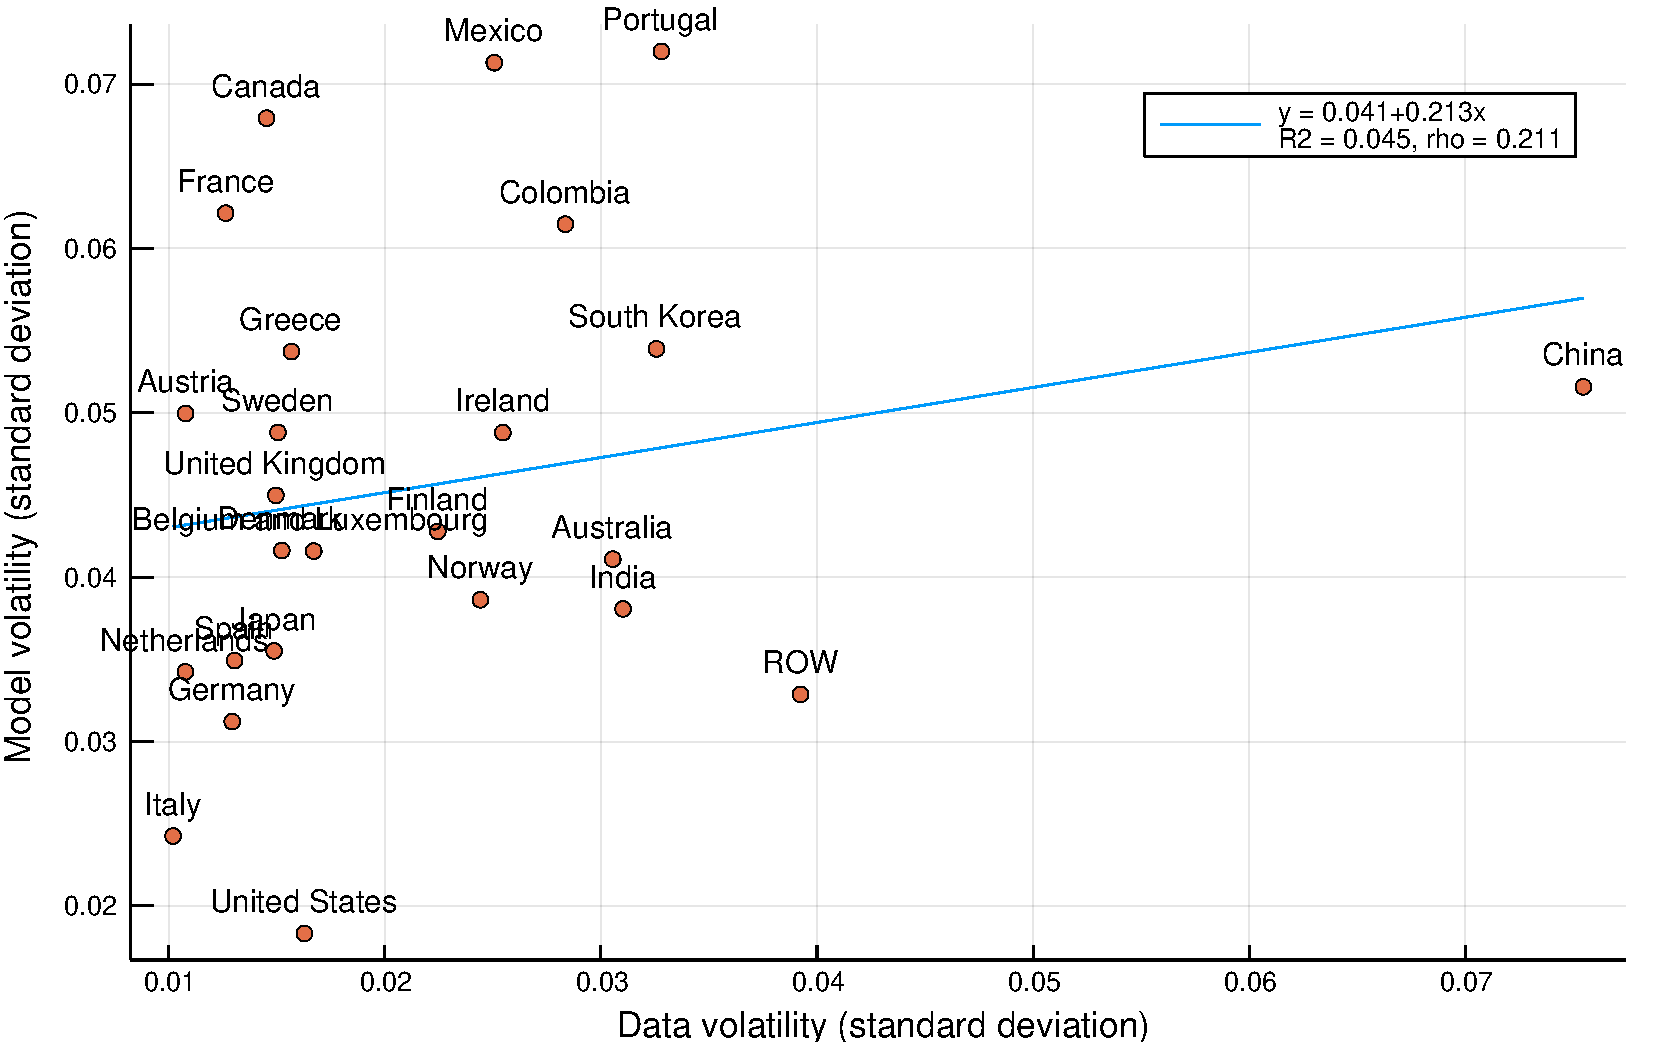
\includegraphics[width=\linewidth]{CES2-model-data.pdf}
\caption{GDP volatility in the data and in the model calibrated to $\sigma=2$}
\end{figure}

As an alternative calibration, we use the price index formula for the Cobb-Douglas specification,
\[
P_{nJt} = (P_{0t}PWT_{nt}/P_{n.t})^{1/\nu_{Jt}}
\]
with
\[
P_{n.t} \equiv \prod_{j=1}^{J-1}P_{njt}^{\nu_{jt}}.
\]
The benefit of this formula is that it does not depend on the noisily measured country-specific expenditure shares. This leads to the same calibrated productivity process as under the Cobb-Douglas scenario ($\sigma=1$). This provides a much better fit with the data (Figure 2).

\begin{figure}
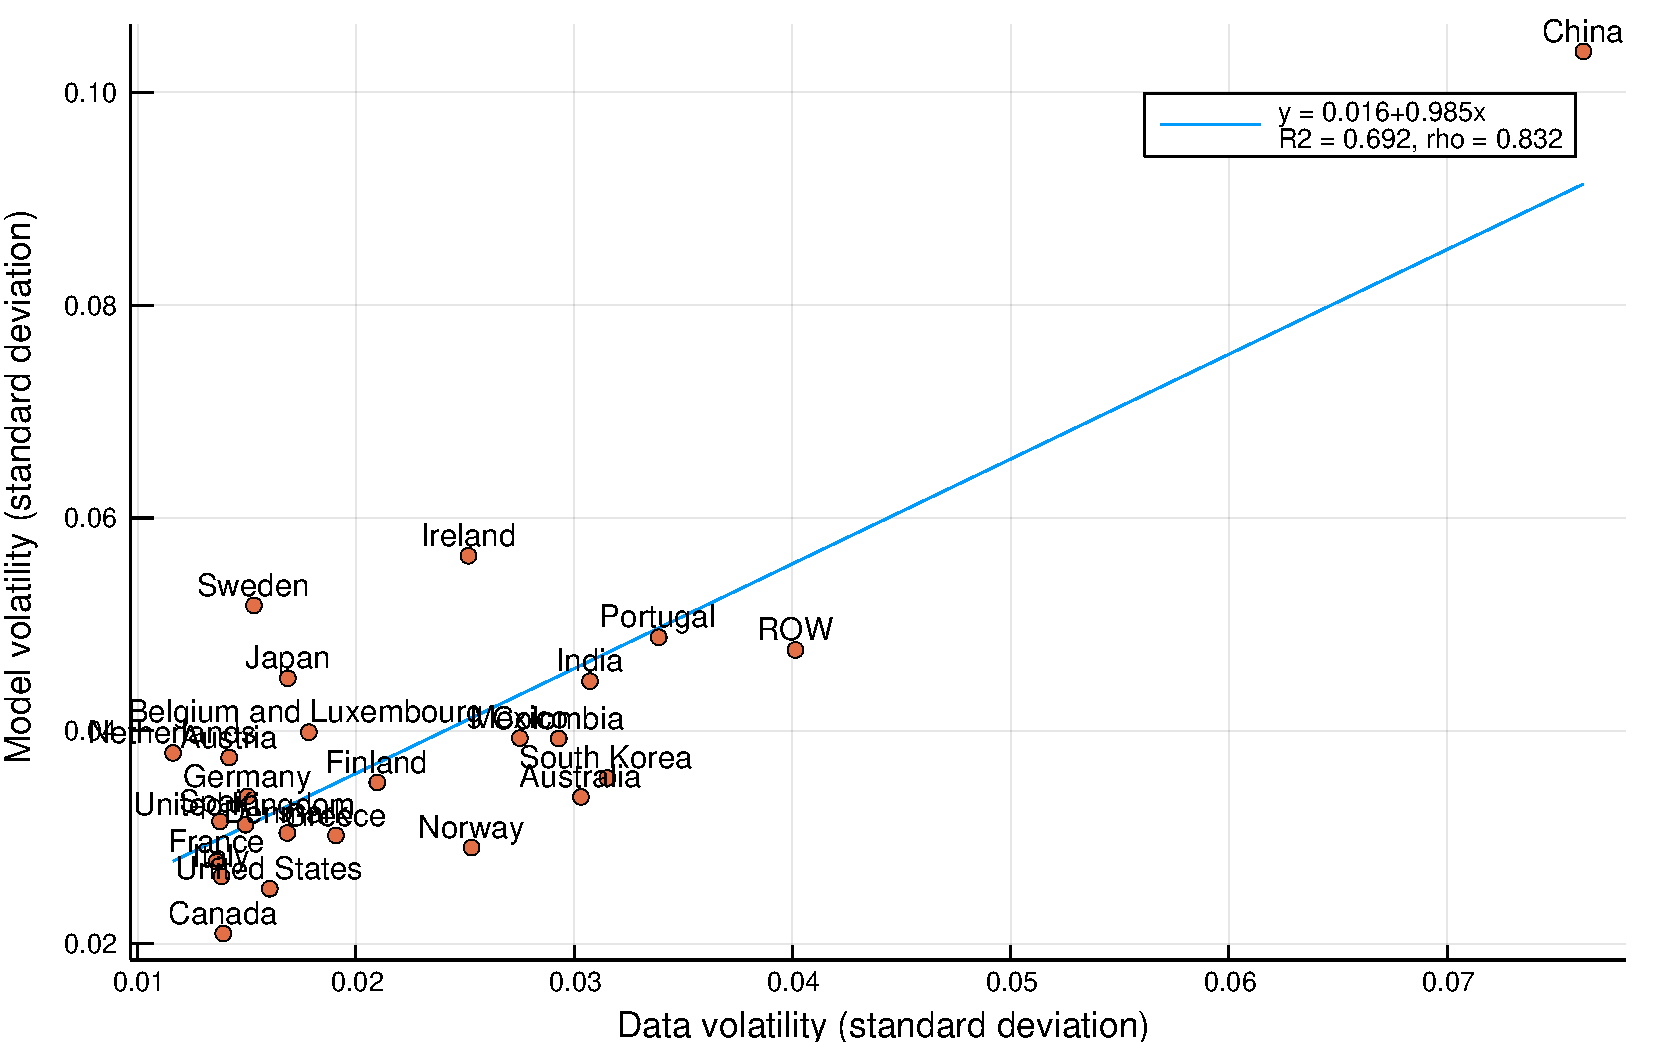
\includegraphics[width=\linewidth]{EOS2-model-data.pdf}
\caption{GDP volatility in the data and in the model with $\sigma=2$ but productivity calibrated to Cobb-Douglas case}
\end{figure}

\subsection{Calibrating US productivity}
Import shares are only informative about relative productivities. For a benchmark country, the US, we calibrate productivity to match observed value added data. Using \eqref{eq:wage}, we can express productivity as a function of sectoral wages,
\begin{equation*}\label{eq:value_added}
A_{njt} =
	\xi B_j
	w_{njt}^{\beta_j}
	\varrho_{njt}^{-1}  	
	\prod_{k=1}^J P_{nkt}^{\gamma_{kj}},
\end{equation*}
and
\[
d_{nnjt} = (\varrho_{njt}/P_{njt})^{-\theta}
\]
can be used to express
\[
\varrho_{njt} = P_{njt} d_{nnjt}^{-1/\theta}.
\]
\begin{equation}\label{eq:productivity}
A_{njt} =
	\xi B_j
	d_{nnjt}^{1/\theta}
	(w_{njt}/P_{njt})^{\beta_j}
 	\prod_{k=1}^J (P_{nkt}/P_{njt})^{\gamma_{kj}}.
\end{equation}
Productivity is high when domestic market share is high, when real wages in sector are high, or when real input costs are high.

Using \eqref{eq:varepsilon} to express sectoral wages in the US,
\[
w_{njt} = w_{nt}
\left[
 {\varrho(L_{njt}-L_{njt}^*)}
+\lambda_{nt}
\right],
\]
with the normalization that $L_{nt}=1$.
How do we calibrate this without observing $L_{njt}$? Multiply by $L_{njt}$,
\[
L_{njt}^2 + (\lambda_{nt}/\varrho-L_{njt}^*) L_{njt} - \frac1\varrho
\frac{w_{njt}L_{njt}} {w_nt} = 0.
\]
Solving this quadratic equation,
\[
L_{njt} = \frac12 (L_{njt}^* - \lambda_{nt}/\varrho)
+ \sqrt{\frac14 (L_{njt}^* - \lambda_{nt}/\varrho)^2 + \frac1\varrho V_{njt}},
\]
where $V_{njt}$ is the value added share in sector $j$. Recall that $\lambda_{nt}$ equals the unweighted average wage ratio across sectors, and is approximately one, ignoring Jensen inequality terms. Also, in equilibrium $L_{njt}^*$ is the expected value added share, which can be approximated by the long-run trend.

This helps us calibrate the sectoral labor share as
\[
L_{njt} \approx (L_{njt}^* - 1/\varrho) \left[
\frac12
+\frac12 \sqrt{1 + \frac1\varrho \frac{V_{njt}}{L_{njt}^* - 1/\varrho}}
\right].
\]
Given a set of labor shares, we can calculate wages as $w_{njt} = Y_{njt}/L_{njt}$.

\subsection{Decomposing productivity shocks}
Given a series of productivities calibrated to the data, we decompose productivity into these four components:
\begin{equation}
	\ln A_{njt} = a_{njt}+\lambda_{jt} + \mu_{nt} +  \varepsilon_{njt}.
\end{equation}
The first term is a Baxter-King trend. The second is a global sector shock, calculated as the $(j,t)$ average of productivity deviations across countries. The third term is calculated as a weighted average of remaining shocks within a country-year. (Weighting is necessary because otherwise idiosyncratic shock of services, the larges sector, would dominate fluctuations in all countries.) The last term is a residual.

The parameter vector $\rho$ and $\sigma$ is estimated using simple OLS. Shocks $u$ are drawn for iid standard normal distribution.
\end{document}
